\documentclass[10pt]{article}
\usepackage[T1]{fontenc}\usepackage{lmodern,amsmath,amssymb,graphicx,hyperref}
\usepackage[margin=.8in]{geometry}
\setlength{\parindent}{0pt}\setlength{\parskip}{7pt}
\begin{document}
\begin{center}{\Large Fourth-power assembly and shared-profile compatibility}\\[4pt]
Local instance-gate continuation --- 15 November 2026\end{center}
\textbf{Assembly result.} A small generic probe uses existing Mathlib
\texttt{coeff\_one\_add\_X\_pow} and
\texttt{comp\_C\_mul\_X\_coeff} as stated to obtain, for any commutative
semiring $R$ and $s\in R$,
\[
 [H^b](1+sH)^n=\binom nb s^b.
\]
For odd $b$, the fourth-power coefficient is a multiple of four:
$b=1,3$ give coefficient $4s^b$, and $b>4$ gives zero. This is standard
binomial algebra assembled from existing laws, not an arithmetic novelty
or a new study-specific law [pcc:unverified].

\textbf{Compatibility question.} A proposed sufficient extension of the
single-anchor parity argument requires, at selected node $i$,
\[
 m_i\equiv1\pmod4,\qquad m_j\equiv0\pmod4\quad(j<u,\ j\ne i).
\]
Before attempting to apply this at every node, the separate probe asks
whether the \emph{same} $m$ can satisfy these requirements for all $i<u$.
For $u\ge2$, taking $i=0$ requires $m_0\bmod4=1$, while taking $i=1$
requires $m_0\bmod4=0$. The one-node boundary has the constant-one profile.
This is a direct test of the proposed quantified residue contract
[pcc:unverified].

\begin{center}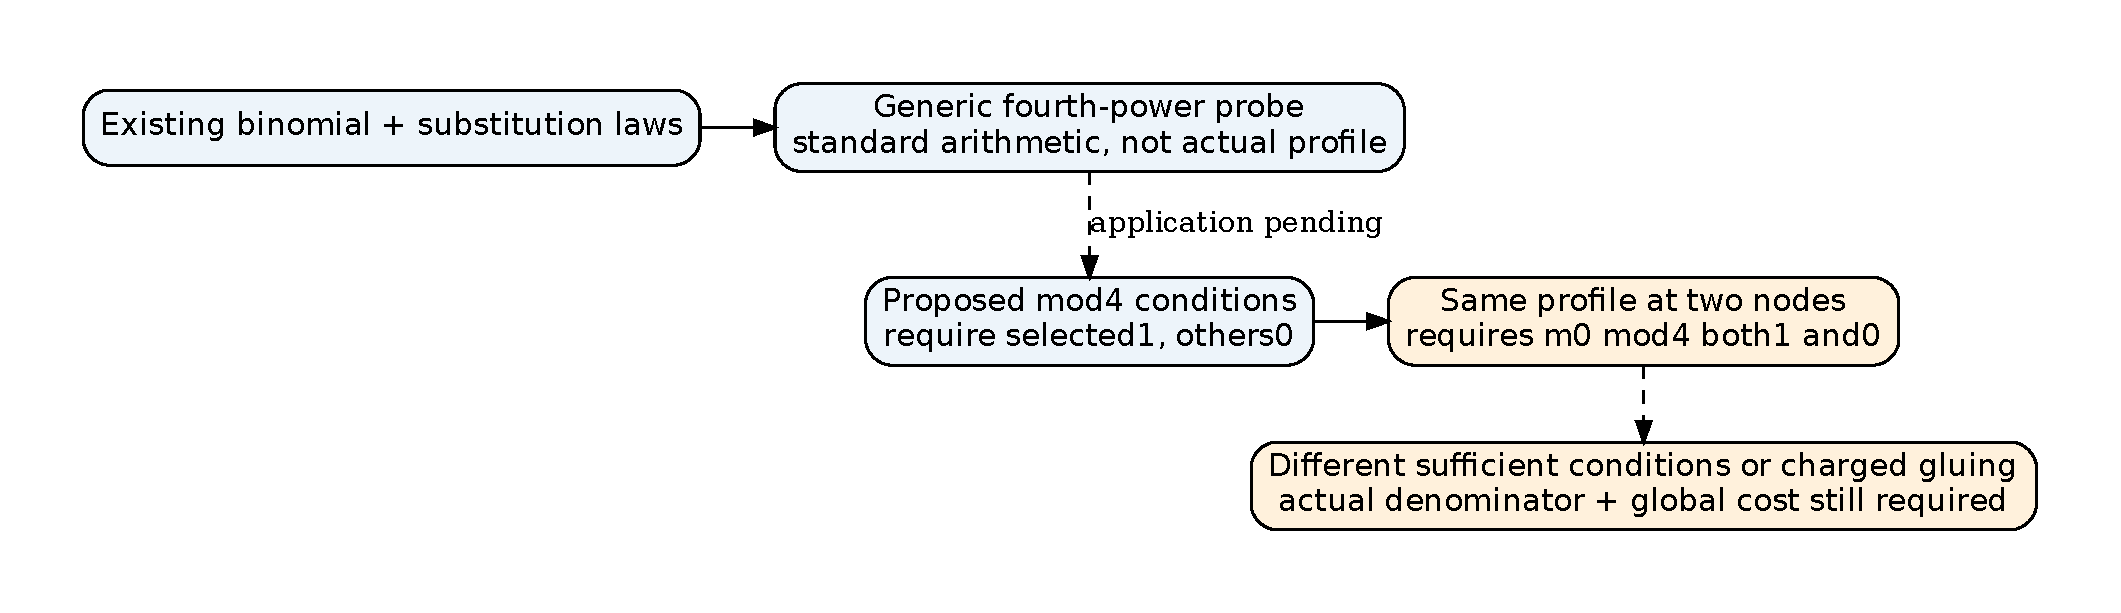
\includegraphics[width=\linewidth,height=1.65in,keepaspectratio]{instance-compatibility-dependencies-001.pdf}\end{center}

\textbf{Evidence scope.} Probe002 compiles with two unnamed generic examples,
exit zero and no warnings. Probe003 adds the compatibility test and one-node
control, also exit zero without warnings. Receipt048 binds both exact runs. Probe001's closed-goal
tactic failure is retained. The six-field instance map lists inherited laws
and the upstream generic candidate. This is assembly evidence, not shared
audit, fresh module coverage or an owned-library promotion
[pcc:unverified].

\textbf{Consequence for the next step.} These congruence conditions have
not been shown necessary for full odd Content2. Rejecting their common-profile
combination cannot exclude other shared profiles, a different denominator
factorization or gluing with fully charged costs. The actual fourth-power
half-slope/denominator application remains open. Do not silently replace
one common auxiliary matrix by a different matrix at each node
[pcc:unverified].

\textbf{Preservation.} Earlier432-statement snapshot, all raw failures,
claims and report pins remain exact. New files only. Publication remains
withheld because remote protected ledger history changed; independent local
mathematics remains possible. No native, timing, scaling, paid/cloud or
attack experiment was run.
\end{document}
